\subsection{Emulated Deadline-Aware Duplication}
\label{sec:dup}
This subsection is new in this report. It measures what the forecasts buy a multipath scheduler (script \texttt{fr\_scheduler.py}). We emulate deadline-aware packet duplication on the test sessions of the four satellite links, with the satellite path as primary and the 5G path of the same direction as backup. At time $t$ the scheduler plans the packets that it will send at $t+h$, $h\in\{0.2,\dots,3\}$\,s. A packet on the primary misses its deadline $D$ if the measured RTT at $t+h$ exceeds $D$, which we set to the 90th percentile of the calibration-session RTT (\SchedDSLDL\,ms on Starlink DL). The scheduler duplicates a packet on the backup when its forecast bound exceeds $D$. We count the share of duplicated packets, which costs backup capacity, and the share of packets that are late and were not duplicated (misses). The backup meets the downlink deadlines in all but \BackupDLmax\% of the 5G DL samples. The 5G UL exceeds the Starlink UL deadline in \BackupQULSL\% of its samples. If the two paths are independent, this raises the miss rate of the S2S-E bound on Starlink UL from \BackupSSmissSLUL\% to \BackupSSmissCorrSLUL\% and that of DS2S-E from \BackupDSmissSLUL\% to \BackupDSmissCorrSLUL\%.

\begin{figure}[H]
  \centering
  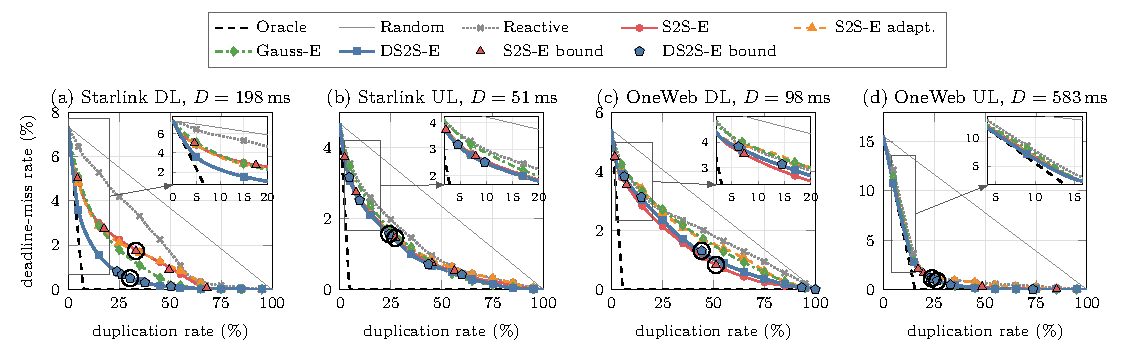
\includegraphics[width=\linewidth]{figs_pdf/fr_scheduler.pdf}
  \caption{Deadline-aware duplication on the test sessions: share of late, non-duplicated packets against the share of duplicated packets, pooled over 0.2--3\,s ($D$: 90th percentile of the calibration-session RTT). Curves sweep the knob of each policy. Markers: one-sided bounds calibrated at levels of 0.80 to 0.99, circled at 0.95. Insets: low duplication. S2S-E adapt.\ scales its margin by the input volatility.}
  \label{fig:sched}
\end{figure}

\paragraph{Deployable comparison.} Each policy has one knob, and sweeping it traces a curve in Fig.~\ref{fig:sched}. A deployed scheduler must set the knob in advance. For S2S-E we use the one-sided 95\% conformal upper bound calibrated on the calibration sessions. For DS2S-E we set the knob on the calibration sessions so that its miss rate there equals that of the S2S-E bound. On Starlink DL, the S2S-E bound duplicates \SchedSSdupSLDL\% of the packets and misses \SchedSSmissSLDL\%. DS2S-E duplicates \SchedDSdupSLDL\% and misses \SchedDSmissSLDL\%, which is \SchedSaveSLDL\% less duplication (95\% CI \SchedSaveSLDLlo{} to \SchedSaveSLDLhi\%) with no more misses. On Starlink UL and OneWeb UL the two schedulers tie (duplication change \SchedSaveSLUL\% and \SchedSaveOWUL\%). On OneWeb DL, DS2S-E needs \SchedDSdupCurveOWDL\% duplication to reach the miss rate of the S2S-E bound, which duplicates \SchedSSdupOWDL\%, and with its knob set on the calibration sessions it misses \SchedDSmissOWDL\% of the packets against \SchedSSmissOWDL\%. Every forecaster with the anchored decoder loses there, including the point forecaster S2S-AE-E. The loss therefore comes from the decoder family and not from the distributional output.

\paragraph{Where the gain comes from.} With the same inputs and decoder, the point forecaster S2S-AE-E needs \SchedFFdupSLDL\% duplication at the miss rate of the S2S-E bound, and DS2S-E needs \SchedDSdupCurveSLDL\% (S2S-E: \SchedSSdupCurveSLDL\%). About half of the gain thus comes from the new inputs and decoder and half from the predictive distribution. With both knobs set on the calibration sessions, DS2S-E needs \SchedSaveFFSLDL\% less duplication than S2S-AE-E. \GaussSchedSentence{} Fig.~\ref{fig:schedheat} breaks the comparison down by deadline and lead time. On Starlink DL the saving is largest for deadlines between the 90th and the 97.5th percentile and at short lead times. It shrinks for the 99th percentile, which lies beyond the 97.5\% quantile that DS2S-E describes. On OneWeb DL the loss is largest at short lead times and strict deadlines.

\begin{figure}[H]
  \centering
  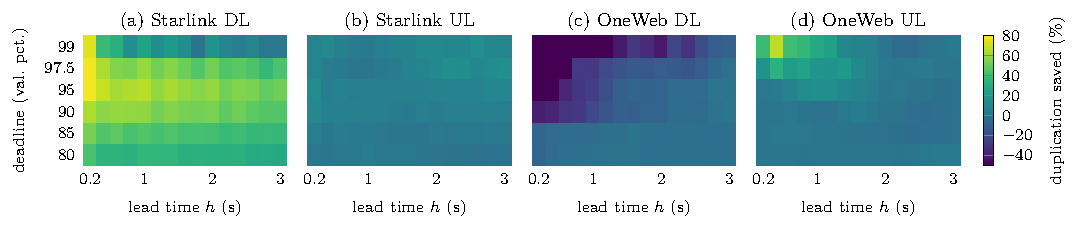
\includegraphics[width=\linewidth]{figs_pdf/fr_scheduler_heat.pdf}
  \caption{Duplication saved by DS2S-E against S2S-E (\%) when 90\% of the late packets must be protected, per deadline (percentile of the calibration-session RTT) and lead time. Values below $-50\%$ are clipped.}
  \label{fig:schedheat}
\end{figure}

\paragraph{Same mean, different risk.} Fig.~\ref{fig:risk} shows what a point forecast misses. It groups the test windows by the S2S-E mean forecast and, within each group, by the spread that DS2S-E predicts. At the same mean forecast of \RiskMeanLo{} to \RiskMeanHi\,ms on Starlink DL, \RiskLowPct\% of the packets are late when DS2S-E predicts a narrow spread and \RiskHighPct\% when it predicts a wide one. A scheduler that sees only the mean must treat these windows alike.

\begin{figure}[H]
  \centering
  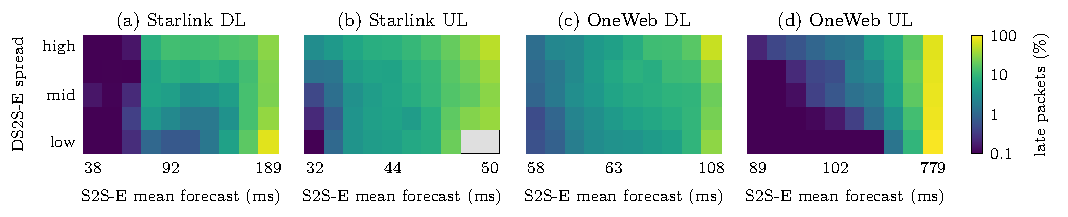
\includegraphics[width=\linewidth]{figs_pdf/fr_scheduler_risk.pdf}
  \caption{Same mean, different risk. Share of late packets (log color scale) when the test windows are grouped by the S2S-E mean forecast (deciles, x) and, within each decile, by the predicted DS2S-E spread $\hat{q}_{0.975}-\hat{q}_{0.5}$ (quintiles, y).}
  \label{fig:risk}
\end{figure}

\paragraph{Caveats.} The curves sweep each knob on the test windows, like an ROC curve. Only the bound-against-bound comparison above is deployable. The conformal guarantee of a bound holds on average and only if calibration and test sessions are exchangeable. On the test sessions the one-sided 95\% bounds covered \BoundCovLo{} to \BoundCovHi{} of the RTT values. The satellite and 5G sessions were not recorded at the same time, so the emulation assumes independent paths.
